\documentclass[aspectratio=169,10pt]{beamer}

\usetheme{Madrid}
\usecolortheme{seahorse}
\usefonttheme{professionalfonts}

\usepackage{amsmath,amssymb,amsthm}
\usepackage{mathtools}
\usepackage{listings}
\usepackage{xcolor}
\usepackage{booktabs}
\usepackage{graphicx}
\usepackage{bm}

\graphicspath{{figures/}}

%% Python style
\lstdefinestyle{python}{
  language=Python,
  basicstyle=\ttfamily\scriptsize,
  keywordstyle=\color{blue!80!black}\bfseries,
  stringstyle=\color{orange!80!black},
  commentstyle=\color{green!50!black}\itshape,
  numberstyle=\tiny\color{gray},
  numbers=left, stepnumber=1,
  frame=single, breaklines=true,
  showstringspaces=false, tabsize=4,
  backgroundcolor=\color{gray!7},
}

\title[MC Theory -- Ch.4]{Lectures on Monte Carlo Theory}
\subtitle{Chapter 4: Simulation Output Analysis: Independent Replications}
\author{Based on Leskel\"{a} \& Vihola}
\date{}

\setbeamertemplate{navigation symbols}{}
\setbeamertemplate{footline}[frame number]

\begin{document}

% ------------------------------------------------------------------ title
\begin{frame}
  \titlepage
\end{frame}

% ------------------------------------------------------------------ TOC
\begin{frame}{Chapter Outline}
  \tableofcontents
\end{frame}

\section{4.1 Estimation of $I$}
\section{4.2 Estimation of $k(I)$ -- Delta Method}
\section{4.3 Estimators of a Quantile}
\section{4.4 Absolute vs Relative Errors}
\section{4.5 Conclusions}

%% ==================================================================
%% SECTION 4.1
%% ==================================================================

\begin{frame}[allowframebreaks]{Chapter Introduction}

  \begin{block}{The Fundamental Problem}
    We aim to estimate $I = \mathbb{E}Y$, where $Y$ is a random variable with
    $\mathbb{E}Y^2 < \infty$ and variance $\sigma_Y^2$.
    We simulate a sample $Y_1, Y_2, \ldots, Y_R$ of i.i.d.\ random variables.
  \end{block}

  \textbf{Two types of errors:}
  \begin{itemize}
    \item \textbf{Absolute error:} $|\hat{I} - I|$, measures the magnitude.
    \item \textbf{Relative error:} $|\hat{I}/I - 1| = |\hat{I} - I|/I$, evaluates error relative to true value.
  \end{itemize}

  \bigskip
  \textbf{Error control conditions} (for $\varepsilon, \delta \in (0,1)$):
  \begin{align*}
    \text{(E1) Absolute: } & \mathbb{P}(|\hat{I} - I| \geq \varepsilon) \leq \delta \\
    \text{(E2) Relative: } & \mathbb{P}(|\hat{I}/I - 1| \geq \varepsilon) \leq \delta
  \end{align*}

  Equivalently:
  \begin{align*}
    \text{(E1'): } & \mathbb{P}(|\hat{I} - I| \leq \varepsilon) \geq 1-\delta \\
    \text{(E2'): } & \mathbb{P}(|\hat{I} - I| \leq \varepsilon I) \geq 1-\delta
  \end{align*}

  \bigskip
  This chapter establishes the \emph{fundamental relationship} between:
  \begin{itemize}
    \item Required precision $b$
    \item Number of replications $R$
    \item Variability $\sigma_Y^2$
  \end{itemize}
\end{frame}

%% ---- 4.1.1 One-dimensional case
\begin{frame}[allowframebreaks]{4.1.1 One-Dimensional Case: Estimator and CLT}

  \begin{block}{Sample Mean Estimator}
    \[
      \hat{Y}_R = \frac{1}{R} \sum_{j=1}^{R} Y_j
    \]
    where $Y_1, \ldots, Y_R$ are i.i.d.\ replications of $Y$ with $\mathbb{E}Y = I$.
  \end{block}

  \textbf{Properties:}
  \begin{itemize}
    \item \textbf{Unbiased:} $\mathbb{E}\hat{Y}_R = I$
    \item \textbf{Strongly consistent:} $\hat{Y}_R \to I$ with probability 1 as $R \to \infty$
    \item \textbf{Weak consistency:} $\mathbb{P}(|\hat{Y}_R - I| \geq b) \to 0$ for any $b > 0$
  \end{itemize}

  \bigskip
  \begin{block}{Chebyshev-Based Error Bound (Remark 4.1.1)}
    Using Chebyshev's inequality:
    \[
      b_R = \frac{1}{\alpha^{1/2}} \frac{\sigma_Y}{\sqrt{R}}
    \]
    which means $b_R = O(R^{-1/2})$.
    \medskip
    \\
    \textit{Symbols:} $b_R$ = error bound, $\alpha$ = significance level, $\sigma_Y$ = std.\ dev.\ of $Y$, $R$ = replications.
  \end{block}

  \framebreak

  \begin{block}{Central Limit Theorem (CLT)}
    If $Y_1, \ldots, Y_R$ are i.i.d.\ with $\sigma_Y = \sqrt{\text{Var}\,Y_j} < \infty$, then as $R \to \infty$:
    \[
      \mathbb{P}\!\left(\sum_{j=1}^{R} \frac{Y_j - I}{\sigma_Y \sqrt{R}} \leq x\right) \to \Phi(x)
    \]
    where $\Phi(x)$ is the standard normal CDF. Equivalently:
    \[
      \sqrt{R}(\hat{Y}_R - I) \xrightarrow{\mathcal{D}} \mathcal{N}(0, \sigma_Y^2)
    \]
  \end{block}

  \begin{block}{Fundamental Relationship (Eq.\ 1.6)}
    \[
      b = z_{1-\alpha/2} \frac{\sigma_Y}{\sqrt{R}}
    \]
    where $z_{1-\alpha/2} = \Phi^{-1}(1 - \alpha/2)$ is the $(1-\alpha/2)$-quantile of $\mathcal{N}(0,1)$.
    \medskip
    \\
    \textit{Symbols:} $b$ = half-width of CI, $z_{1-\alpha/2}$ = normal quantile, $\sigma_Y$ = std.\ dev., $R$ = sample size.
  \end{block}

  \framebreak

  \begin{block}{Required Number of Replications}
    To achieve prescribed error $b$ at confidence level $1-\alpha$:
    \[
      R = z_{1-\alpha/2}^2 \frac{\sigma_Y^2}{b^2}
    \]
  \end{block}

  \textbf{Common case} ($\alpha = 0.05$, $z_{1-\alpha/2} = z_{0.975} = 1.96$):
  \[
    b = \frac{1.96\,\sigma_Y}{\sqrt{R}}, \qquad R = \frac{1.96^2\,\sigma_Y^2}{b^2}
  \]

  \bigskip
  \textbf{Chebyshev vs CLT comparison (Remark 4.1.5):}
  \[
    \frac{b^{\rm CLT}}{b^{\rm Ch}} = z_{1-\alpha/2}\,\alpha^{1/2} = 43.82\%
    \quad (\alpha = 0.05)
  \]
  Using CLT requires only $\approx 19.2\%$ of the replications needed by Chebyshev's bound.

\end{frame}

%% ---- Sample variance
\begin{frame}[allowframebreaks]{4.1.1 Sample Variance and Confidence Interval}

  In practice $\sigma_Y^2$ is unknown; we replace it with the \textbf{sample variance}:

  \begin{block}{Unbiased Sample Variance}
    \[
      \hat{S}_R^2 = \frac{1}{R-1} \sum_{j=1}^{R} (Y_j - \hat{Y}_R)^2
    \]
    $\mathbb{E}\hat{S}_R^2 = \sigma_Y^2$ (unbiased), strongly consistent.
  \end{block}

  \begin{block}{$1-\alpha$ Confidence Interval (Eq.\ 1.9)}
    \[
      \left(\hat{Y}_R - z_{1-\alpha/2}\frac{\hat{S}_R}{\sqrt{R}},\;
             \hat{Y}_R + z_{1-\alpha/2}\frac{\hat{S}_R}{\sqrt{R}}\right)
    \]
    \textit{Interpretation:} Contains the true $I$ with approximate probability $1-\alpha$.
  \end{block}

  \textbf{Recursive update formulas} (online computation):
  \[
    \hat{Y}_{R+1} = \hat{Y}_R + \frac{Y_{R+1} - \hat{Y}_R}{R+1}
  \]
  \[
    \hat{\sigma}_{R+1}^2 = \hat{\sigma}_R^2 + (\hat{Y}_R)^2 - (\hat{Y}_{R+1})^2
      + \frac{(Y_{R+1})^2 - \hat{\sigma}_R^2 - (\hat{Y}_R)^2}{R+1}
  \]

\end{frame}

%% ---- Examples 4.1.6, 4.1.7
\begin{frame}[allowframebreaks]{4.1.1 Examples: Estimating $\pi$}

  \begin{block}{Example 4.1.6 -- Indicator (Hit-or-Miss) Estimator}
    Take $Y = 4\cdot\mathbf{1}(U_1^2 + U_2^2 \leq 1)$ where $U_1, U_2 \sim \mathcal{U}[0,1]$ i.i.d.
    \[
      \hat{Y}_R = \frac{1}{R}\sum_{j=1}^R Y_j, \quad Y_j = 4\cdot\mathbf{1}(U_{2j-1}^2 + U_{2j}^2 \leq 1)
    \]
    $\mathbb{E}Y = \pi$, $\text{Var}\,Y = 16(\pi/4)(1-\pi/4) \approx 2.6968$.\\
    For 1st digit accuracy ($b=0.5$): $R \approx 1.96^2 \cdot 2.6968/0.25 \approx 42$.\\
    For 2nd digit ($b=0.05$): $R \approx 4144$.
  \end{block}

  \begin{block}{Example 4.1.7 -- Smooth Estimator}
    Take $Y = 4\sqrt{1 - U^2}$ where $U \sim \mathcal{U}[0,1]$, so $\mathbb{E}Y = \pi$.
    \[
      \text{Var}\,Y = \frac{32}{3} - \pi^2 \approx 0.797
    \]
    For 1st digit ($b=0.5$): $R \approx 12$.\quad For 2nd digit ($b=0.05$): $R \approx 1224$.\\
    \medskip
    Variance $\approx 3.38\times$ smaller than Example 4.1.6!
  \end{block}

  \begin{center}
    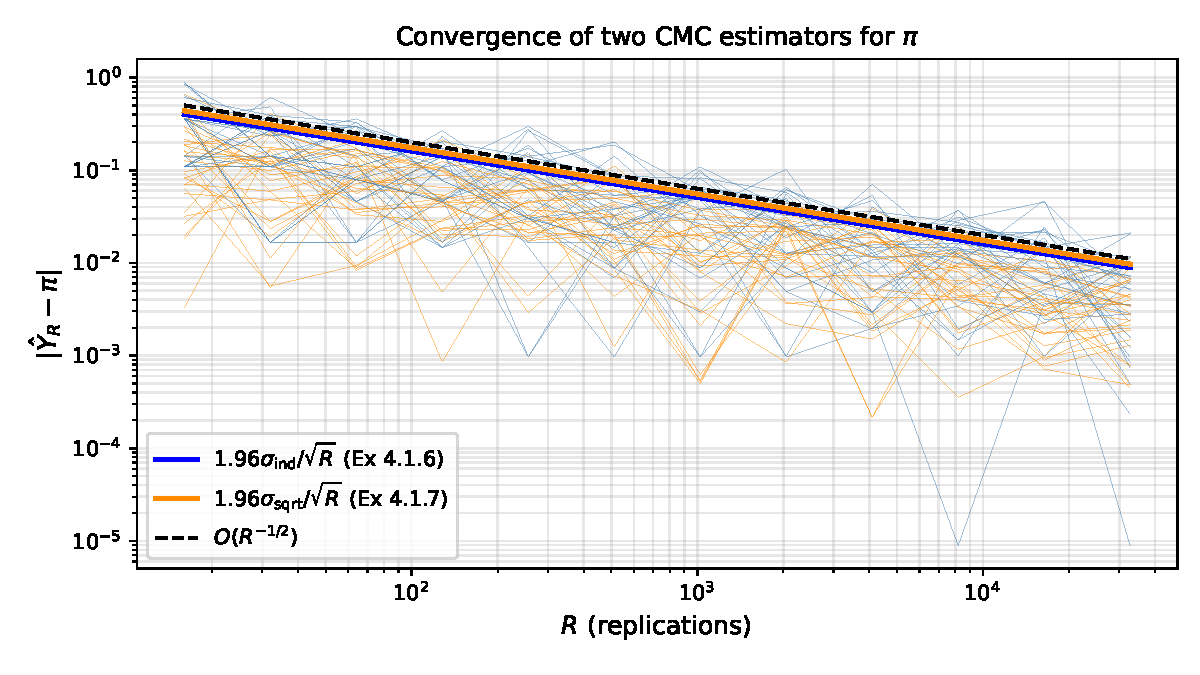
\includegraphics[width=0.82\textwidth]{fig_pi_convergence}
  \end{center}

\end{frame}

%% ---- Hit-or-miss
\begin{frame}{4.1.1 Crude Monte Carlo and Hit-or-Miss}

  \begin{columns}
    \begin{column}{0.48\textwidth}
      \begin{block}{Crude Monte Carlo (CMC)}
        For $I = \int_B k(x)\,dx$ with $\text{Vol}(B)=1$:
        \[
          \hat{Y}_R^{\rm CMC} = \frac{1}{R}\sum_{j=1}^R k(V_j)
        \]
        where $V_j \sim \mathcal{U}(B)$ i.i.d.
      \end{block}
      \begin{block}{Hit-or-Miss (HoM)}
        For $0 \leq k(x) \leq 1$, define:
        \[
          Y' = \mathbf{1}(k(U_1) > U_2)
        \]
        Then $\mathbb{E}Y' = \int_0^1 k(u)\,du = I$.
        \[
          \hat{Y}_R^{\rm HoM} = \frac{1}{R}\sum_{j=1}^R Y'_j
        \]
        HoM requires $2R$ uniforms; generally less efficient than CMC.
      \end{block}
    \end{column}
    \begin{column}{0.50\textwidth}
      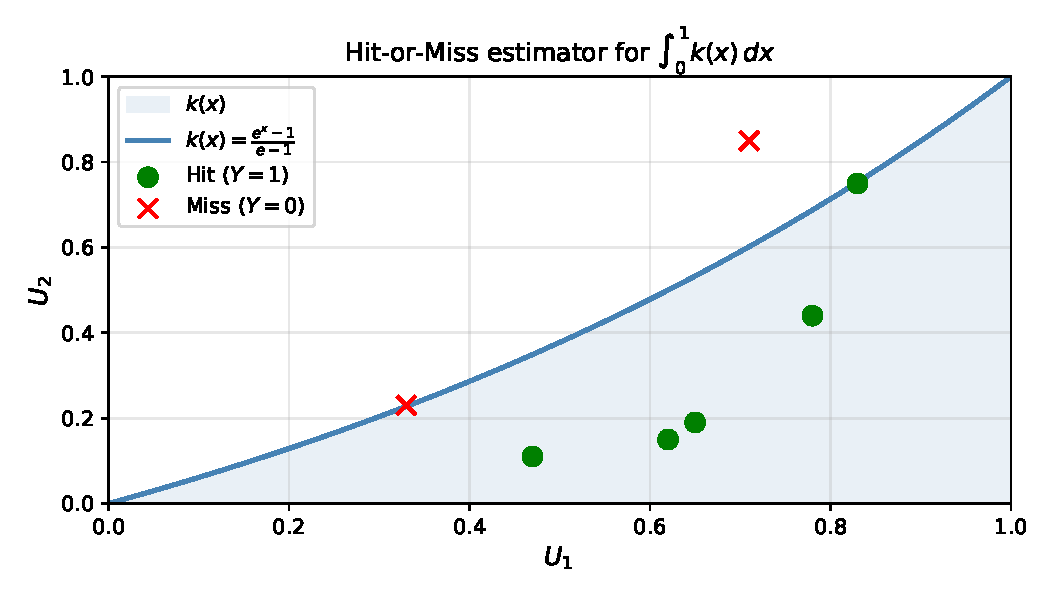
\includegraphics[width=\textwidth]{fig_hit_or_miss}
    \end{column}
  \end{columns}

\end{frame}

%% ---- CLT confidence interval illustration
\begin{frame}{4.1.1 CLT: Distribution of $\hat{Y}_R$}
  \begin{center}
    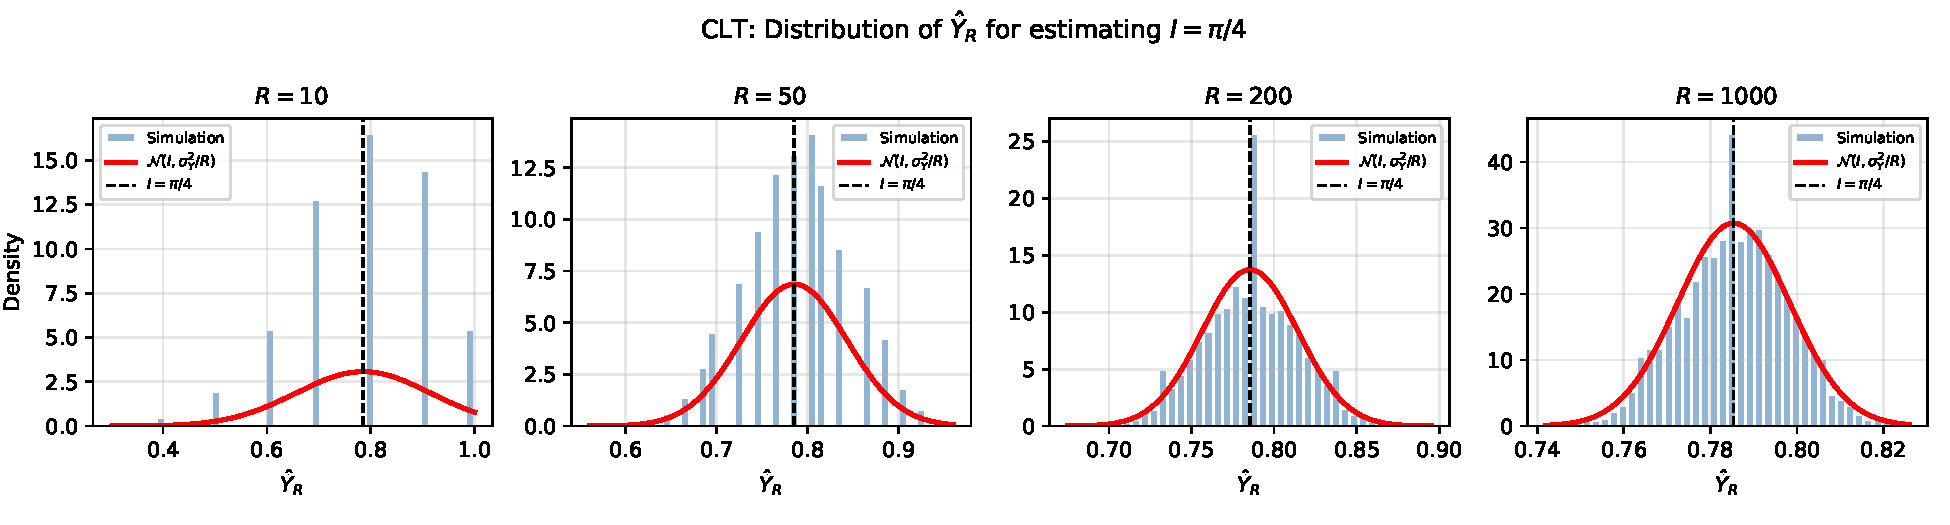
\includegraphics[width=0.95\textwidth]{fig_clt_convergence}
  \end{center}
  \begin{itemize}
    \item As $R$ increases, $\hat{Y}_R$ concentrates around $I = \pi/4$
    \item Distribution approaches $\mathcal{N}(I, \sigma_Y^2/R)$ (red curve)
    \item CI coverage confirmed empirically
  \end{itemize}
\end{frame}

%% ---- CI coverage figure
\begin{frame}{4.1.1 Confidence Interval Coverage}
  \begin{center}
    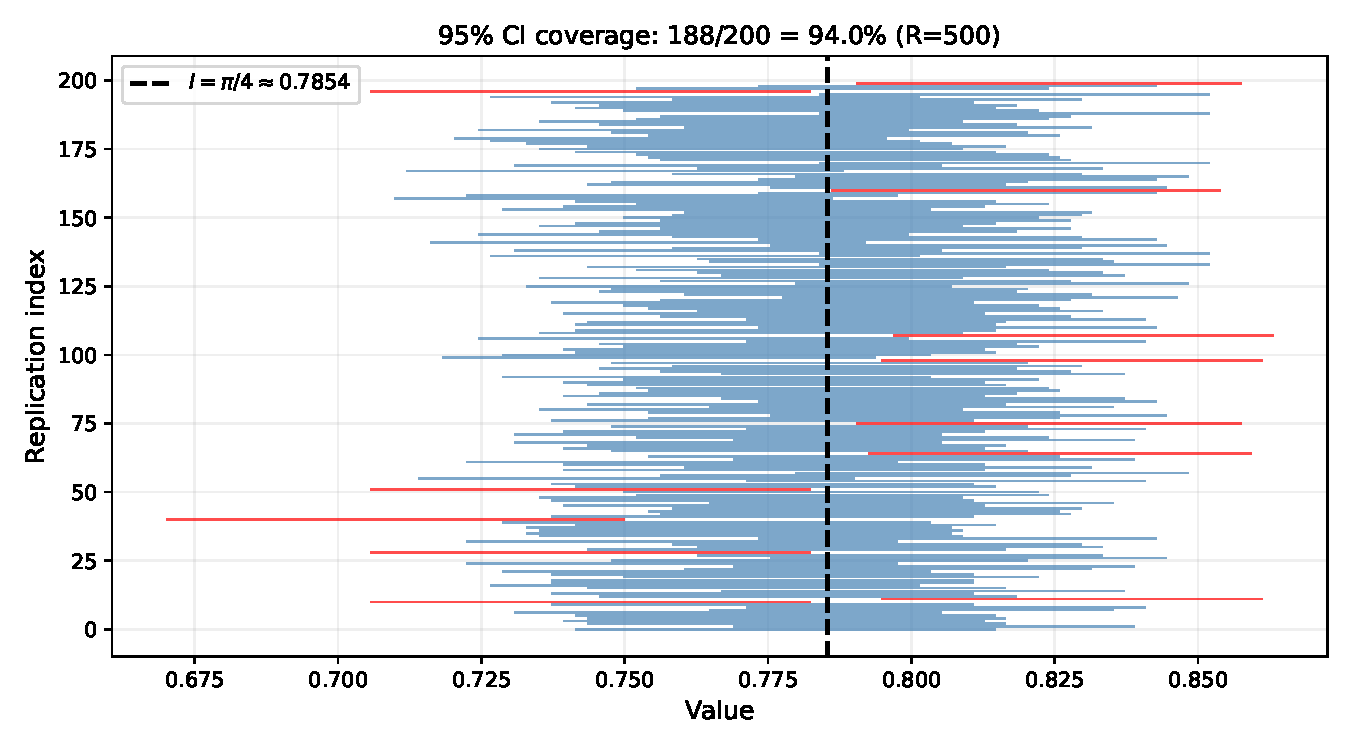
\includegraphics[width=0.72\textwidth]{fig_ci_coverage}
  \end{center}
  \begin{itemize}
    \item 200 independent 95\% CIs for $I = \pi/4$ with $R = 500$
    \item Blue: CI contains $I$ (correct); Red: CI misses $I$
    \item Coverage close to nominal 95\%
  \end{itemize}
\end{frame}

%% ---- Python code: one-dimensional CI
\begin{frame}[fragile]{4.1.1 Python: Computing a Confidence Interval}
\begin{lstlisting}[style=python]
import numpy as np
from scipy import stats

def estimate_pi_ci(R, alpha=0.05, seed=42):
    """Estimate pi using hit-or-miss MC and compute 95% CI."""
    rng = np.random.default_rng(seed)
    U = rng.random((R, 2))
    # Y_j = 4 * 1(U1^2 + U2^2 <= 1)
    Y = 4.0 * (U[:, 0]**2 + U[:, 1]**2 <= 1).astype(float)

    Y_bar = Y.mean()            # estimator
    S2 = Y.var(ddof=1)          # unbiased sample variance
    S = np.sqrt(S2)

    z = stats.norm.ppf(1 - alpha / 2)  # z_{1-alpha/2}
    margin = z * S / np.sqrt(R)

    ci_lo = Y_bar - margin
    ci_hi = Y_bar + margin
    return Y_bar, ci_lo, ci_hi

# Example: R = 10000, alpha = 0.05
Y_bar, lo, hi = estimate_pi_ci(R=10_000)
print(f"Estimate: {Y_bar:.4f}")
print(f"95% CI: ({lo:.4f}, {hi:.4f})")
print(f"True pi: {np.pi:.4f}")
# Output: Estimate: 3.1464, 95% CI: (3.1142, 3.1786)
\end{lstlisting}
\end{frame}

%% ==================================================================
%% 4.1.2 Multidimensional Case
%% ==================================================================

\begin{frame}[allowframebreaks]{4.1.2 Multidimensional Case}

  We aim to estimate $\mathbf{I} = (I^{(1)}, \ldots, I^{(d)})^T = \mathbb{E}\mathbf{Y}$
  where $\mathbf{Y} = (Y^{(1)}, \ldots, Y^{(d)})^T \in \mathbb{R}^d$.

  \begin{block}{Vector Sample Mean Estimator}
    \[
      \hat{\mathbf{Y}}_R = \frac{1}{R}\sum_{j=1}^R \mathbf{Y}_j,
      \qquad \mathbf{Y}_j = \begin{pmatrix} Y_j^{(1)} \\ \vdots \\ Y_j^{(d)} \end{pmatrix}
    \]
  \end{block}

  \begin{block}{Multivariate CLT}
    Let $\boldsymbol{\Sigma}_{\mathbf{Y}} = \mathbb{E}[(\mathbf{Y}-\mathbf{I})(\mathbf{Y}-\mathbf{I})^T]$
    be the covariance matrix of $\mathbf{Y}$. Then:
    \[
      \sqrt{R}(\hat{\mathbf{Y}}_R - \mathbf{I}) \xrightarrow{\mathcal{D}} \mathcal{N}\!\left(\mathbf{0}, \boldsymbol{\Sigma}_{\mathbf{Y}}\right)
    \]
    so $\hat{\mathbf{Y}}_R \approx \mathcal{N}\!\left(\mathbf{I},\, \frac{1}{R}\boldsymbol{\Sigma}_{\mathbf{Y}}\right)$.
  \end{block}

\end{frame}

%% ---- 4.1.2.1 Facts about Multivariate Normal
\begin{frame}[allowframebreaks]{4.1.2.1 Facts about the Multivariate Normal Distribution}

  \begin{block}{Definition}
    $\mathbf{X} \sim \mathcal{N}(\boldsymbol{\mu}, \boldsymbol{\Sigma})$ with
    $\boldsymbol{\Sigma}$ nonsingular $d\times d$ covariance matrix.
  \end{block}

  \begin{block}{Spectral Decomposition}
    $\boldsymbol{\Sigma} = \mathbf{F}\boldsymbol{\Lambda}\mathbf{F}^T = \sum_{i=1}^d \lambda_i \mathbf{f}_i\mathbf{f}_i^T$
    where:
    \begin{itemize}
      \item $\lambda_1, \ldots, \lambda_d > 0$: eigenvalues of $\boldsymbol{\Sigma}$
      \item $\mathbf{f}_1, \ldots, \mathbf{f}_d$: orthonormal eigenvectors
      \item $\boldsymbol{\Sigma}^{1/2} = \mathbf{F}\boldsymbol{\Lambda}^{1/2}\mathbf{F}^T$ (square root)
    \end{itemize}
  \end{block}

  \begin{block}{Proposition 4.1.13 -- Key Properties}
    For $\mathbf{X} \sim \mathcal{N}(\boldsymbol{\mu}, \boldsymbol{\Sigma})$ with $\boldsymbol{\Sigma} = \mathbf{A}\mathbf{A}^T$:
    \begin{enumerate}[(a)]
      \item $\mathbf{Z} = \mathbf{A}^{-1}(\mathbf{X} - \boldsymbol{\mu}) \sim \mathcal{N}(\mathbf{0}, \mathbf{Id}_d)$
      \item $(\mathbf{X}-\boldsymbol{\mu})^T\boldsymbol{\Sigma}^{-1}(\mathbf{X}-\boldsymbol{\mu}) \sim \chi_d^2$
        (chi-square with $d$ d.f.)
    \end{enumerate}
  \end{block}

  \framebreak

  \textbf{Consequence:} For $\mathbf{X} \sim \mathcal{N}(\boldsymbol{\mu}, \boldsymbol{\Sigma})$:
  \[
    \mathbb{P}\!\left((\mathbf{X}-\boldsymbol{\mu})^T\boldsymbol{\Sigma}^{-1}(\mathbf{X}-\boldsymbol{\mu})
      \leq q_{1-\alpha}(\chi_d^2)\right) \approx 1-\alpha
  \]
  where $q_{1-\alpha}(\chi_d^2)$ is the $(1-\alpha)$-quantile of $\chi^2_d$.

  \bigskip
  \textbf{Example values ($\alpha = 0.05$):}
  \begin{center}
    \begin{tabular}{ccc}
      \toprule
      $d$ & $q_{0.95}(\chi_d^2)$ & Ellipsoid ``radius'' \\
      \midrule
      1   & 3.841 & 1.96 \\
      2   & 5.991 & -- \\
      5   & 11.07 & -- \\
      \bottomrule
    \end{tabular}
  \end{center}

\end{frame}

%% ---- 4.1.2.2 Shapes of Confidence Regions
\begin{frame}[allowframebreaks]{4.1.2.2 Shapes of Confidence Regions}

  For $\mathbf{X} \sim \mathcal{N}(\boldsymbol{\mu}, \boldsymbol{\Sigma})$, three standard confidence region shapes:

  \begin{block}{Ellipsoid (Tightest)}
    \[
      \mathcal{C}^{\rm el} = \left\{\mathbf{x} : \mathbf{x}^T\boldsymbol{\Sigma}^{-1}\mathbf{x}
        \leq q_{1-\alpha}(\chi_d^2)\right\}
    \]
    Centered at $\mathbf{0}$ with principal axes $\sqrt{q_{1-\alpha}(\chi_d^2)\lambda_i}\,\mathbf{f}_i$.
  \end{block}

  \begin{block}{Parallelogram (via Hypercube)}
    Define hypercube $\mathcal{H} = (-z,z)^d$ where $z = \Phi^{-1}\!\left(\frac{\sqrt[d]{1-\alpha}+1}{2}\right)$.
    The confidence parallelogram is:
    \[
      \mathcal{C}^{\rm par} = \boldsymbol{\Sigma}^{1/2}\mathcal{H} + \boldsymbol{\mu}
    \]
    with vertices $\boldsymbol{\Sigma}^{1/2}\mathbf{v}_i + \boldsymbol{\mu}$ for $\mathbf{v}_i = (\pm z, \ldots, \pm z)$.
  \end{block}

  \begin{block}{Rectangle (Conservative, via Sidak)}
    By independence of coordinates of $\boldsymbol{\Sigma}^{-1/2}(\mathbf{X}-\boldsymbol{\mu})$:
    \[
      \mathcal{C}^{\rm rec} = [-c_1, c_1] \times \cdots \times [-c_d, c_d],
      \quad c_i = \sigma_i\,\Phi^{-1}\!\left(\frac{1+\sqrt[d]{1-\alpha}}{2}\right)
    \]
    This uses the \emph{Sidak inequality}: satisfies $\mathbb{P}(\mathbf{X} \in \mathcal{C}^{\rm rec}) \geq 1-\alpha$.
  \end{block}

  \framebreak

  \begin{center}
    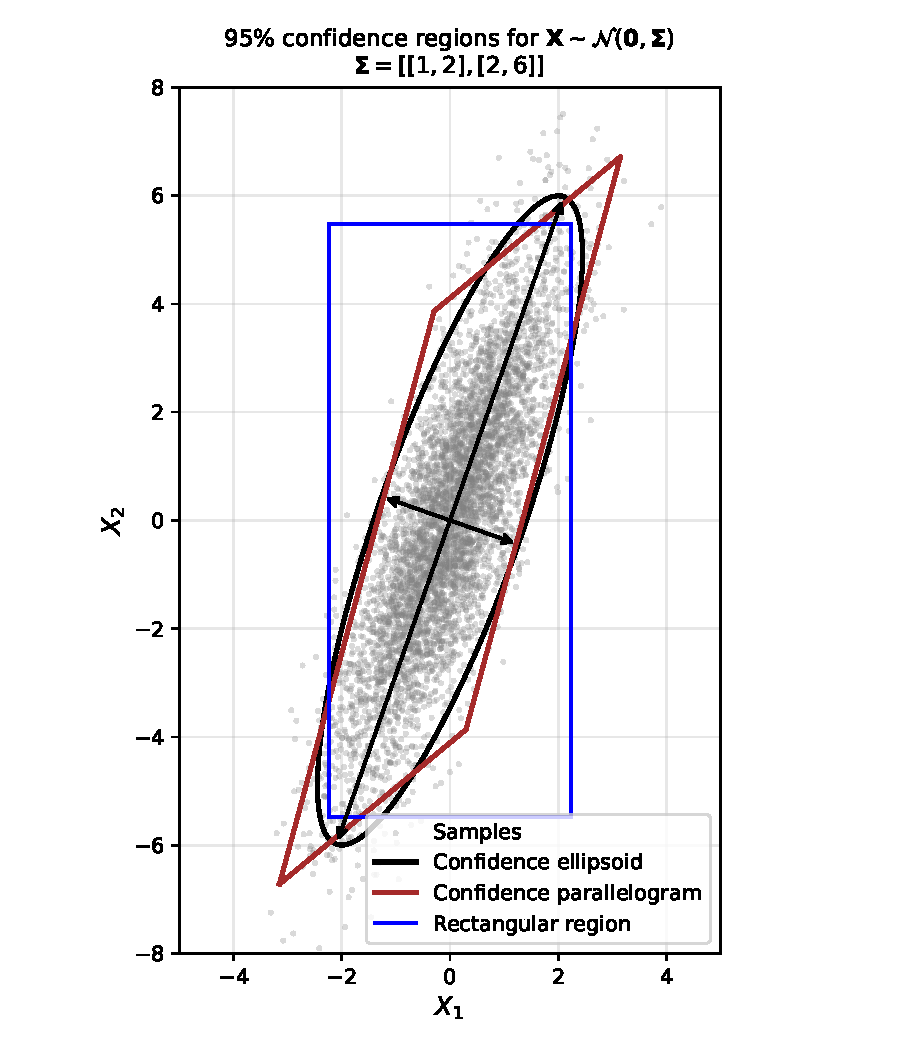
\includegraphics[width=0.52\textwidth]{fig_conf_regions_2d}
  \end{center}

  \textbf{Example 4.1.14:} $\boldsymbol{\Sigma} = \begin{pmatrix}1 & 2 \\ 2 & 6\end{pmatrix}$,
  $\alpha = 0.05$, $d=2$.
  \begin{itemize}
    \item Eigenvalues: $\lambda_1 = (7+\sqrt{41})/2 \approx 6.70$, $\lambda_2 \approx 0.30$
    \item Ellipsoid axes lengths: $\sqrt{q_{0.95}\lambda_1} \approx 6.34$,
      $\sqrt{q_{0.95}\lambda_2} \approx 1.34$
    \item Rectangle: $\mathcal{C}^{\rm rec} = [-2.2365,\,2.2365] \times [-5.4782,\,5.4782]$
  \end{itemize}

\end{frame}

%% ---- 4.1.2.3 Confidence regions for Y_R
\begin{frame}[allowframebreaks]{4.1.2.3 Confidence Regions for $\hat{\mathbf{Y}}_R$ of $\mathbf{I}$}

  We now construct confidence regions for the \emph{estimator} $\hat{\mathbf{Y}}_R$
  (centered at $\hat{\mathbf{Y}}_R$, covering $\mathbf{I}$).

  \begin{block}{Estimated Confidence Ellipsoid}
    \textbf{Procedure:}
    \begin{enumerate}
      \item Compute $\hat{\mathbf{Y}}_R = \frac{1}{R}\sum_{k=1}^R \mathbf{Y}_k$
      \item Compute sample covariance $\hat{\mathbf{S}}_R^2 = \frac{1}{R-1}\sum_{k=1}^R
        (\mathbf{Y}_k - \hat{\mathbf{Y}}_R)(\mathbf{Y}_k - \hat{\mathbf{Y}}_R)^T$
      \item Compute eigendecomposition of $\hat{\mathbf{S}}_R^2$: eigenvalues $\lambda_i$, eigenvectors $\mathbf{f}_i$
      \item Principal axes of ellipsoid:
        $\sqrt{\frac{q_{1-\alpha}(\chi_d^2)\,\lambda_i}{R}}\,\mathbf{f}_i$
      \item Ellipsoid: $\hat{\mathbf{Y}}_R + \mathcal{C}$
    \end{enumerate}
  \end{block}

  \textbf{Note (Remark 4.1.15):} Replacing $\boldsymbol{\Sigma}_{\mathbf{Y}}$ by
  $\hat{\mathbf{S}}_R^2$ means the statistic $R(\hat{\mathbf{Y}}_R - \mathbf{I})^T(\hat{\mathbf{S}}_R^2)^{-1}(\hat{\mathbf{Y}}_R - \mathbf{I})$
  follows Hotelling's $T^2$-distribution. For large $R$, this is approximately $\chi^2_d$.

  \framebreak

  \textbf{Example 4.1.16 -- Heights/Weights dataset}
  ($R = 1000$, $d = 2$: height $I^{(1)}$, weight $I^{(2)}$ of 18-year-olds):

  \begin{itemize}
    \item $\hat{Y}_R^{(1)} = 127.48$,\quad $\hat{S}_R^{(1)} = 11.80$
    \item $\hat{Y}_R^{(2)} = 68.05$,\quad $\hat{S}_R^{(2)} = 1.94$
    \item 95\% CI for height: $\mathbb{P}(126.75 \leq I^{(1)} \leq 128.21) = 95\%$
    \item 95\% CI for weight: $\mathbb{P}(67.93 \leq I^{(2)} \leq 68.17) = 95\%$
  \end{itemize}

  \begin{block}{Sample Covariance Matrix}
    \[
      \hat{\mathbf{S}}_R^2 = \begin{pmatrix} 139.29 & 11.40 \\ 11.40 & 3.75 \end{pmatrix},
      \quad \lambda_1 = 140.24,\;\lambda_2 = 2.79
    \]
  \end{block}

\end{frame}

%% ---- Python code: multivariate CI
\begin{frame}[fragile]{4.1.2 Python: Multivariate Confidence Ellipsoid}
\begin{lstlisting}[style=python]
import numpy as np
from scipy.stats import chi2

def conf_ellipsoid(Y_samples, alpha=0.05):
    """Compute confidence ellipsoid for mean of d-dim samples."""
    R, d = Y_samples.shape
    Y_bar = Y_samples.mean(axis=0)          # sample mean (d-vector)

    # Sample covariance matrix
    diff = Y_samples - Y_bar
    S2 = (diff.T @ diff) / (R - 1)

    # Eigendecomposition
    eigvals, eigvecs = np.linalg.eigh(S2)
    q = chi2.ppf(1 - alpha, df=d)           # chi-square quantile

    # Axis lengths of confidence ellipsoid
    axis_lengths = np.sqrt(q * eigvals / R)
    return Y_bar, axis_lengths, eigvecs, S2

# Simulate 2D example: I = (2.0, 3.0), Sigma = [[1,0.5],[0.5,2]]
rng = np.random.default_rng(42)
Sigma = np.array([[1., 0.5], [0.5, 2.]])
L = np.linalg.cholesky(Sigma)
R = 500
Y = (L @ rng.standard_normal((2, R))).T + np.array([2.0, 3.0])

Y_bar, axes, vecs, S2 = conf_ellipsoid(Y, alpha=0.05)
print(f"Estimated mean: {Y_bar}")
print(f"Ellipsoid axis lengths: {axes}")
\end{lstlisting}
\end{frame}

%% ==================================================================
%% SECTION 4.2
%% ==================================================================

\begin{frame}[allowframebreaks]{4.2 Estimation of $k(I)$ -- Overview}

  \begin{block}{Problem Setup}
    We aim to estimate $z = k(I)$ (or $z = k(\mathbf{I})$), where:
    \begin{itemize}
      \item $k : \mathbb{R}^d \to \mathbb{R}$ is a prescribed continuous function
      \item $I = \mathbb{E}Y$ (or $\mathbf{I} = \mathbb{E}\mathbf{Y}$) is computable via simulation
      \item $\hat{X}_R$ is a strongly consistent estimator of $I$
    \end{itemize}
    The natural estimator is:
    \[
      \hat{Z}_R = k(\hat{X}_R)
    \]
  \end{block}

  \textbf{Key quantity -- Asymptotic Variance:}
  \[
    \varsigma^2 = \lim_{R\to\infty} R\,\text{Var}\hat{Z}_R
    \quad\text{(also called the TAVC)}
  \]

  \begin{block}{Example: $k(x) = x$ (identity)}
    $\hat{Z}_R = \hat{Y}_R$, $\varsigma^2 = \text{Var}\,Y = \sigma_Y^2$.
    This reduces to Section 4.1.
  \end{block}

  \bigskip
  \textbf{Important:} $k(\hat{Y}_R)$ is generally \emph{biased} even when $\hat{Y}_R$ is unbiased.

\end{frame}

%% ---- 4.2.1 Case X_R = Y_R
\begin{frame}[allowframebreaks]{4.2.1 The Case $\hat{X}_R = \hat{Y}_R$ -- Delta Method}

  \begin{block}{Proposition 4.2.1 -- Delta Method (1D)}
    Let $Y_1, Y_2, \ldots$ be i.i.d., $\hat{Y}_R = \frac{1}{R}\sum Y_j$, and suppose $k$ is
    continuously differentiable in a neighborhood of $I = \mathbb{E}Y$. Then:
    \[
      \sqrt{R}\bigl(k(\hat{Y}_R) - k(I)\bigr) \xrightarrow{\mathcal{D}} \mathcal{N}(0, \varsigma^2)
    \]
    where:
    \[
      \varsigma^2 = k'(I)^2\,\sigma_Y^2 = \lim_{R\to\infty} R\,\text{Var}\hat{Z}_R
    \]
    \textit{Symbols:} $k'(I)$ = derivative of $k$ at $I$, $\sigma_Y^2 = \text{Var}\,Y$.
  \end{block}

  \textbf{Proof sketch (Delta Method):} Taylor expansion:
  \[
    k(x) - k(I) = k'(I)(x-I) + o(x-I)
  \]
  So $\sqrt{R}(k(\hat{Y}_R) - k(I)) \approx k'(I)\sqrt{R}(\hat{Y}_R - I) \xrightarrow{\mathcal{D}} \mathcal{N}(0, k'(I)^2\sigma_Y^2)$.

  \framebreak

  \begin{block}{Practical Confidence Interval for $k(I)$ (Eq.\ 2.3)}
    \[
      \left(k(\hat{Y}_R) - z_{1-\alpha/2}\frac{\hat{S}_R\,k'(\hat{Y}_R)}{\sqrt{R}},\;
             k(\hat{Y}_R) + z_{1-\alpha/2}\frac{\hat{S}_R\,k'(\hat{Y}_R)}{\sqrt{R}}\right)
    \]
    where $\hat{S}_R^2$ is the sample variance and $k'(\hat{Y}_R)$ approximates $k'(I)$.
  \end{block}

  \begin{block}{Example 4.2.2 -- Insurance Net Premium}
    $\Pi = r\frac{\mathbb{E}e^{-rT}}{1 - \mathbb{E}e^{-rT}} = k(I)$
    where $I = \mathbb{E}e^{-rT}$ and $k(x) = \frac{rx}{1-x}$, $k'(x) = \frac{r}{(1-x)^2}$.

    Confidence interval:
    \[
      \left(k(\hat{Y}_R) - \frac{z_{1-\alpha/2}\,r\hat{S}_R}{(1-\hat{Y}_R)^2\sqrt{R}},\;
             k(\hat{Y}_R) + \frac{z_{1-\alpha/2}\,r\hat{S}_R}{(1-\hat{Y}_R)^2\sqrt{R}}\right)
    \]
  \end{block}

  \begin{center}
    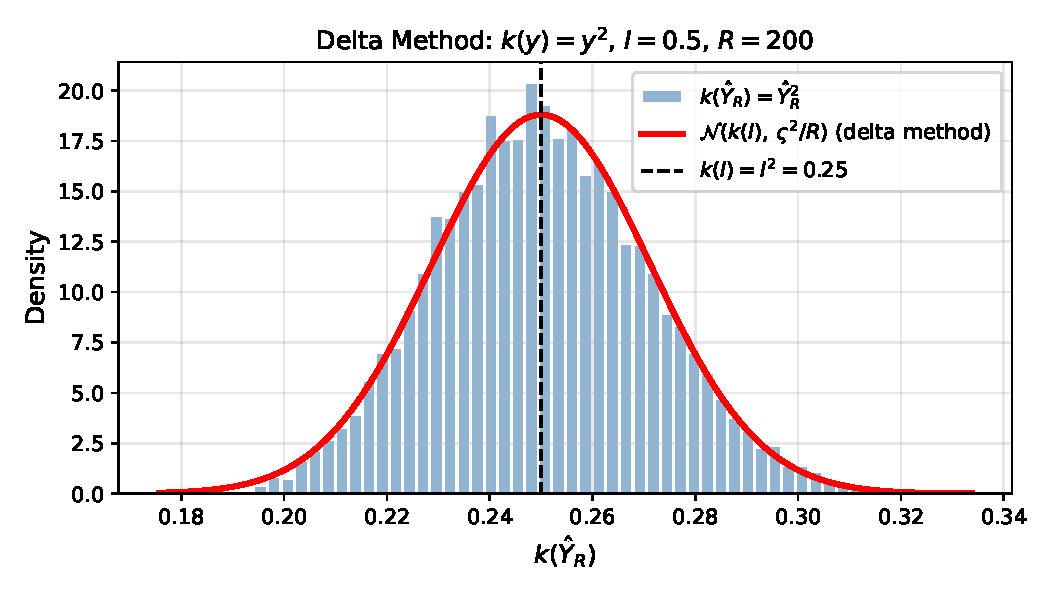
\includegraphics[width=0.55\textwidth]{fig_delta_method}
  \end{center}

\end{frame}

%% ---- Multidimensional delta method
\begin{frame}[allowframebreaks]{4.2.1 Multidimensional Delta Method}

  \begin{block}{Proposition 4.2.3 -- 2D Case}
    Let $\mathbf{Y}_1, \mathbf{Y}_2, \ldots$ be i.i.d.\ replications of $\mathbf{Y} = (Y^{(1)}, Y^{(2)})^T$,
    and $k(y_1, y_2)$ continuously differentiable at $\mathbf{I} = (I^{(1)}, I^{(2)})$.
    For $\hat{Z}_R = k(\hat{\mathbf{Y}}_R)$:
    \[
      \sqrt{R}(k(\hat{\mathbf{Y}}_R) - k(\mathbf{I})) \xrightarrow{\mathcal{D}} \mathcal{N}(0, \varsigma^2)
    \]
    where:
    \[
      \varsigma^2 = (k'_{y_1})^2\boldsymbol{\Sigma}_{\mathbf{Y}}(1,1)
        + (k'_{y_2})^2\boldsymbol{\Sigma}_{\mathbf{Y}}(2,2)
        + 2k'_{y_1}k'_{y_2}\boldsymbol{\Sigma}_{\mathbf{Y}}(1,2)
    \]
    (all partial derivatives evaluated at $\mathbf{I}$).
  \end{block}

  \begin{block}{General Case -- Proposition 4.2.8}
    For $k : \mathbb{R}^d \to \mathbb{R}$ continuously differentiable at $\mathbf{I}$:
    \[
      \sqrt{R}(k(\hat{\mathbf{Y}}_R) - k(\mathbf{I})) \xrightarrow{\mathcal{D}} \mathcal{N}(0, \varsigma^2)
    \]
    \[
      \varsigma^2 = \nabla k(\mathbf{I})\,\boldsymbol{\Sigma}_{\mathbf{Y}}\,(\nabla k(\mathbf{I}))^T
        = \sum_{i,j=1}^d k^{(i)}(\mathbf{I})\,k^{(j)}(\mathbf{I})\,\boldsymbol{\Sigma}_{\mathbf{Y}}(i,j)
    \]
  \end{block}

  \framebreak

  \textbf{Practical CI} for $z = k(\mathbf{I})$ at level $1-\alpha$:
  \[
    k(\hat{\mathbf{Y}}_R) \pm 1.96\,\frac{\hat{\varsigma}}{\sqrt{R}}
  \]
  where estimated asymptotic variance:
  \[
    \hat{\varsigma}^2 = \sum_{i,j=1}^d k^{(i)}(\hat{\mathbf{Y}}_R)\,k^{(j)}(\hat{\mathbf{Y}}_R)\,
      \hat{\mathbf{S}}_R^2(i,j)
  \]

  \begin{block}{Example 4.2.5 -- Ratio of Expectations}
    Estimate $z = I^{(1)}/I^{(2)}$ using $k(y_1,y_2) = y_1/y_2$:
    \[
      \hat{Z}_R = \frac{\hat{Y}_R^{(1)}}{\hat{Y}_R^{(2)}},\qquad
      \varsigma^2 = \frac{\mathbb{E}(Y^{(1)} - zY^{(2)})^2}{(I^{(2)})^2}
    \]
    Estimated variance:
    \[
      \widehat{\text{Var}}(\hat{Z}_R) = \frac{1}{R^2(\hat{Y}_R^{(2)})^2}
        \sum_{i=1}^R (Y_i^{(1)} - \hat{Z}_R\,Y_i^{(2)})^2
    \]
  \end{block}

\end{frame}

%% ---- 4.2.2 General Consistent Estimator
\begin{frame}[allowframebreaks]{4.2.2 General Consistent Estimator $\hat{X}_R$}

  Consider a more general strongly consistent estimator $\hat{X}_R$ of $I$ satisfying:
  \begin{enumerate}[(A1)]
    \item $\sqrt{R}(\hat{X}_R - \mathbb{E}\hat{X}_R) \xrightarrow{\mathcal{D}} \mathcal{N}(0, \sigma^2)$,
      where $0 < \sigma^2 < \infty$
    \item $\sqrt{R}(\mathbb{E}\hat{X}_R - I) \to 0$ (asymptotic unbiasedness)
  \end{enumerate}

  \textbf{Result:} Under (A1) and (A2):
  \[
    \sqrt{R}(\hat{X}_R - I) \xrightarrow{\mathcal{D}} \mathcal{N}(0, \sigma^2)
  \]
  and for $\hat{Z}_R = k(\hat{X}_R)$:
  \[
    \sqrt{R}(k(\hat{X}_R) - k(I)) \xrightarrow{\mathcal{D}} \mathcal{N}(0, \varsigma^2),
    \quad \varsigma^2 = k'(I)^2\,\sigma^2
  \]

  \begin{block}{Asymptotic Bias of $\hat{Z}_R$ (Eq.\ 2.17)}
    Under stronger assumption (A2'): $R(\mathbb{E}\hat{X}_R - I) \to \beta^X$, the
    $R^{-1}$-order asymptotic bias of $\hat{Z}_R$ is:
    \[
      \beta^Z = \beta^X k'(I) + \frac{\sigma^2 k''(I)}{2}
    \]
    Bias-corrected estimator: $k(\hat{X}_R) - \beta^Z/R$.
  \end{block}

\end{frame}

%% ---- 4.2.3 MSE
\begin{frame}[allowframebreaks]{4.2.3 Mean Square Error, Bias, and Variance}

  \begin{block}{Bias-Variance Decomposition (MSE)}
    For estimator $\hat{X}_R$ of $I$:
    \[
      \text{MSE}(\hat{X}_R) = \mathbb{E}(\hat{X}_R - I)^2
        = \underbrace{\mathbb{E}(\hat{X}_R - \mathbb{E}\hat{X}_R)^2}_{\text{Variance}}
          + \underbrace{(\mathbb{E}\hat{X}_R - I)^2}_{\text{Bias}^2}
    \]
    This is the \emph{bias-variance decomposition} (Eq.\ 2.19).
  \end{block}

  For large $R$:
  \[
    \text{MSE}(\hat{X}_R) \approx \frac{\varsigma^2}{R} + \frac{\beta^2}{R^2}
  \]
  \begin{itemize}
    \item \textbf{Variance term} $\varsigma^2/R$ dominates for large $R$ (order $R^{-1}$)
    \item \textbf{Bias$^2$ term} $\beta^2/R^2$ is negligible for large $R$ (order $R^{-2}$)
  \end{itemize}

  \begin{center}
    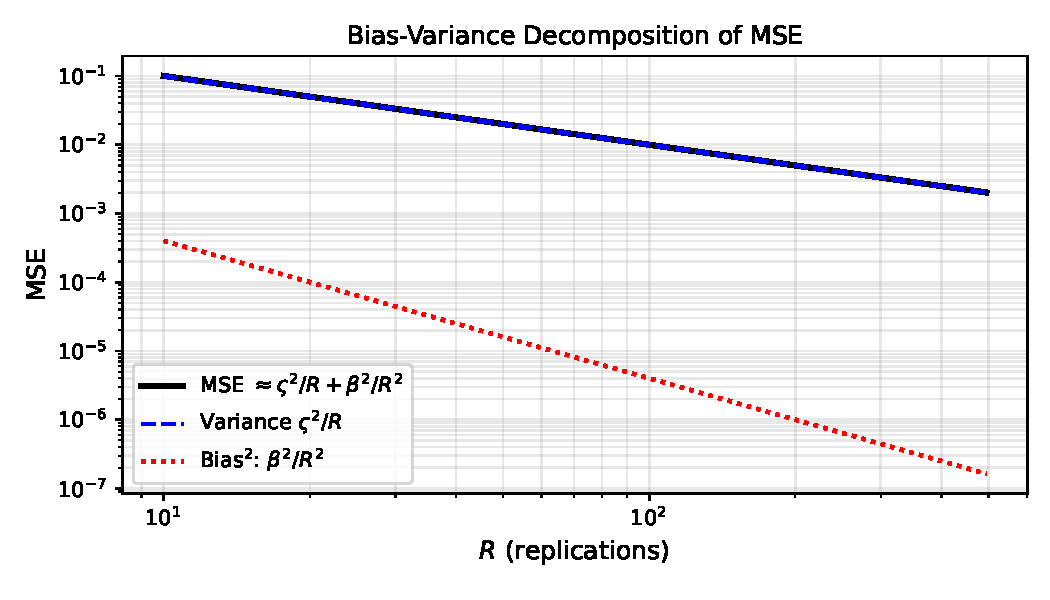
\includegraphics[width=0.65\textwidth]{fig_mse_decomp}
  \end{center}

  \framebreak

  \begin{block}{Rule of Thumb (Remark 4.2.4)}
    Bias corrections are often implemented believing they improve accuracy in small samples.
    However, for large $R$ (typical in Monte Carlo), the standard deviation $\varsigma/\sqrt{R}$
    dominates the bias $\beta/R$, making correction negligible.

    \textbf{Principle:} The standard deviation should dominate the bias for confidence
    intervals to remain meaningful.
  \end{block}

  \begin{block}{Example 4.2.9 -- $k(y) = y^2$}
    For $\hat{Z}_R = \hat{Y}_R^2$:
    \[
      \mathbb{E}(\hat{Y}_R)^2 = (\mathbb{E}Y)^2 + R^{-1}\sigma_Y^2 = k(I) + R^{-1}\sigma_Y^2
    \]
    The asymptotic bias of order $R^{-1}$ is $\beta = \sigma_Y^2/2$
    (from $k''(y) = 2$, since $\beta = k''(I)\sigma_Y^2/2$).
  \end{block}

\end{frame}

%% ---- Python: Delta method CI
\begin{frame}[fragile]{4.2 Python: Delta Method Confidence Interval}
\begin{lstlisting}[style=python]
import numpy as np
from scipy import stats

def delta_method_ci(Y_samples, k_func, k_prime, alpha=0.05):
    """
    Compute CI for k(I) using delta method.

    Parameters
    ----------
    Y_samples : 1D array of i.i.d. realizations of Y (EY = I)
    k_func    : callable, the transformation k
    k_prime   : callable, derivative k'
    """
    R = len(Y_samples)
    Y_bar = Y_samples.mean()         # estimator of I
    S = Y_samples.std(ddof=1)        # sample std dev

    z_est = k_func(Y_bar)            # point estimate of k(I)
    # Asymptotic std dev: |k'(Y_bar)| * S / sqrt(R)
    asymp_std = abs(k_prime(Y_bar)) * S / np.sqrt(R)

    z_q = stats.norm.ppf(1 - alpha / 2)
    return z_est, z_est - z_q * asymp_std, z_est + z_q * asymp_std

# Example: k(y) = y^2, Y ~ N(0.5, 0.09), I=0.5, k(I)=0.25
rng = np.random.default_rng(42)
Y = rng.normal(0.5, 0.3, 1000)
est, lo, hi = delta_method_ci(Y, lambda y: y**2, lambda y: 2*y)
print(f"k(I) estimate: {est:.4f}")
print(f"95% CI: ({lo:.4f}, {hi:.4f})")
print(f"True k(I) = 0.25. Bias: {est - 0.25:.4f}")
# Output: k(I) estimate: 0.2594, 95% CI: (0.2399, 0.2789)
\end{lstlisting}
\end{frame}

%% ==================================================================
%% SECTION 4.3 Quantile Estimation
%% ==================================================================

\begin{frame}[allowframebreaks]{4.3 Estimators of a Quantile}

  \begin{block}{Setup}
    Let $X \sim F$ with density $f$. The $p$-th quantile (for $p \in (0,1)$) is:
    \[
      q_p = F^{\leftarrow}(p) = \inf\{x : F(x) \geq p\}
    \]
    In financial math: $q_p = \text{VaR}_X(p)$ (Value-at-Risk).
  \end{block}

  \begin{block}{Sample Quantile via Order Statistics}
    Given i.i.d.\ sample $X_1, \ldots, X_R$ with order statistics $X_{(1)} \leq \cdots \leq X_{(R)}$:
    \[
      \hat{F}_R^{\leftarrow}(p) = \begin{cases}
        X_{(\lfloor pR\rfloor)} & \text{if } pR \text{ is an integer}\\
        X_{(\lfloor pR\rfloor+1)} & \text{otherwise}
      \end{cases}
    \]
    For simplicity, we use $\hat{q}_p = X_{(\lfloor pR\rfloor)}$.
  \end{block}

  \begin{block}{Proposition 4.3.1 -- Asymptotic Normality of $\hat{q}_p$}
    Assume $f$ is continuous and positive in a neighborhood of $q_p$. Then:
    \begin{enumerate}[(i)]
      \item $\hat{q}_p$ is a strongly consistent estimator of $q_p$
      \item $\sqrt{R}(\hat{q}_p - q_p) \xrightarrow{\mathcal{D}} \mathcal{N}(0, \varsigma^2)$,
        where $\varsigma^2 = \dfrac{p(1-p)}{f(q_p)^2}$
    \end{enumerate}
    \textit{Symbols:} $f(q_p)$ = density at the quantile, $p$ = probability level.
  \end{block}

  \framebreak

  \textbf{Proof sketch:} Based on the Beta distribution of order statistics.
  \begin{itemize}
    \item $U_{(\lfloor Rp\rfloor)} \sim \text{Beta}(\lfloor Rp\rfloor, R - \lfloor Rp\rfloor)$
    \item By Lemma 4.3.3: $\sqrt{R}(U_{\lfloor Rp\rfloor} - p) \xrightarrow{\mathcal{D}} \mathcal{N}(0, p(1-p))$
    \item Apply Taylor expansion: $F^{\leftarrow}(p+x) \approx F^{\leftarrow}(p) + \frac{x}{f(q_p)}$
    \item Combining: $\sqrt{R}(\hat{q}_p - q_p) \xrightarrow{\mathcal{D}} \mathcal{N}(0, p(1-p)/f(q_p)^2)$
  \end{itemize}

  \begin{center}
    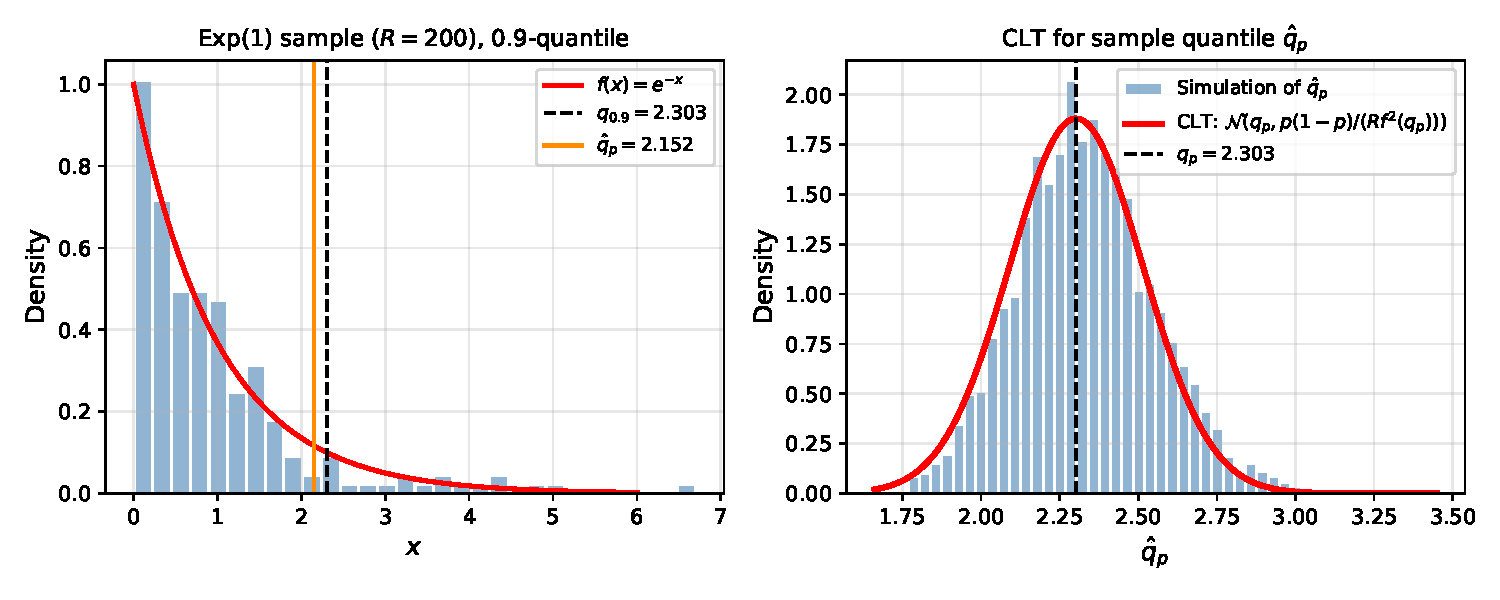
\includegraphics[width=0.8\textwidth]{fig_quantile_estimation}
  \end{center}

\end{frame}

%% ---- 4.3.1 Estimation of 1/f(q_p)
\begin{frame}[allowframebreaks]{4.3.1 Estimation of $1/f(q_p)$ via Order Statistics}

  To construct a practical CI for $q_p$, we need to estimate $1/f(q_p)$.

  \begin{block}{Kernel Estimator (Proposition 4.3.4)}
    Define $Q(p) = F^{-1}(p)$, so $Q'(p) = 1/f(Q(p)) = 1/f(q_p)$.

    Using finite differences with parameter $m = m_R$:
    \[
      \hat{Q}'_{p,R} = \frac{R}{2m}\!\left(X_{(\lfloor pR\rfloor + m)} - X_{(\lfloor pR\rfloor - m + 1)}\right)
    \]

    \textbf{Consistency:} If $f$ has a continuous derivative near $q_p$ and
    $m_R \to \infty$ with $m_R = o(R)$, then $\hat{Q}'_{p,R}$ is strongly consistent.
  \end{block}

  \textbf{Choice of bandwidth} $m_R$:
  \begin{itemize}
    \item Simple rule: $m_R = cR^{1/2}$
    \item MSE-optimal (Bloch-Gastwirth): $m_R = cR^{4/5}$ minimizes
      $\mathbb{E}(\hat{Q}'_{p,R} - Q'(p))^2 \sim \frac{5}{4}\cdot 9^{-1/5}[Q'(p)]^{4/5}[Q''(p)]^{3/5}R^{-2/5}$
  \end{itemize}

  \begin{block}{Confidence Interval for $q_p$}
    Combining Proposition 4.3.1 and $\hat{Q}'_{p,R}$:
    \[
      \hat{q}_p \pm z_{1-\alpha/2}\,\sqrt{\frac{p(1-p)}{R}}\,\hat{Q}'_{p,R}
    \]
  \end{block}

  \framebreak

  \begin{center}
    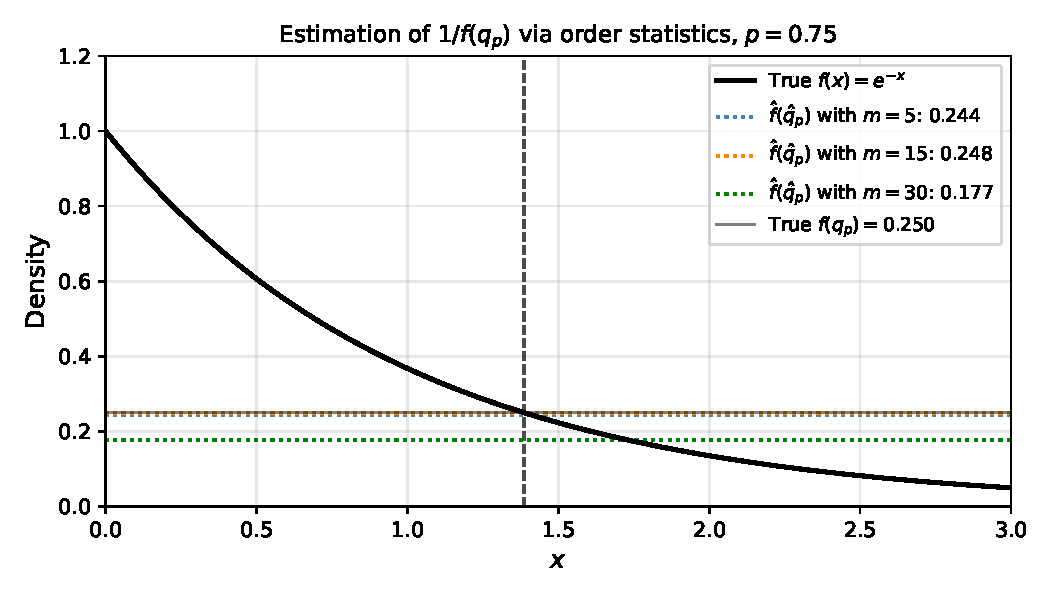
\includegraphics[width=0.7\textwidth]{fig_kde_quantile}
  \end{center}

  \textbf{Example:} $X \sim \text{Exp}(1)$, $p = 0.75$, $R = 500$.
  \begin{itemize}
    \item True quantile: $q_{0.75} = \ln 4 \approx 1.386$
    \item True $f(q_p) = e^{-q_{0.75}} = 0.25$
    \item Different bandwidth choices $m$ give different accuracy
    \item Larger $m$: more smoothing, potentially more bias
  \end{itemize}

\end{frame}

%% ---- Python: quantile CI
\begin{frame}[fragile]{4.3 Python: Sample Quantile and Confidence Interval}
\begin{lstlisting}[style=python]
import numpy as np
from scipy import stats

def quantile_ci(X_samples, p, m=None, alpha=0.05):
    """
    Estimate p-quantile and compute confidence interval.

    Parameters
    ----------
    X_samples : 1D array of i.i.d. samples
    p         : quantile level in (0, 1)
    m         : bandwidth parameter (default: sqrt(R))
    """
    R = len(X_samples)
    X_sorted = np.sort(X_samples)
    idx = int(np.floor(p * R))          # index of sample quantile
    q_hat = X_sorted[idx]               # sample quantile

    if m is None:
        m = max(1, int(np.sqrt(R)))

    lo_idx = max(0, idx - m)
    hi_idx = min(R - 1, idx + m - 1)
    # Estimate 1/f(q_p) via order-stat differences
    Q_prime_hat = R * (X_sorted[hi_idx] - X_sorted[lo_idx]) / (2 * m)

    # Confidence interval
    z_q = stats.norm.ppf(1 - alpha / 2)
    margin = z_q * np.sqrt(p * (1 - p) / R) * Q_prime_hat
    return q_hat, q_hat - margin, q_hat + margin

# Example: X ~ Exp(1), p=0.9, R=500
rng = np.random.default_rng(42)
X = rng.exponential(1.0, 500)
q_hat, lo, hi = quantile_ci(X, p=0.9)
print(f"q_0.9 estimate: {q_hat:.4f}")
print(f"95% CI: ({lo:.4f}, {hi:.4f})")
print(f"True q_0.9 = {-np.log(0.1):.4f}")  # = log(10) ~ 2.303
\end{lstlisting}
\end{frame}

%% ==================================================================
%% SECTION 4.4 Absolute vs Relative Errors
%% ==================================================================

\begin{frame}[allowframebreaks]{4.4 More on Absolute vs Relative Errors}

  \textbf{Recall the error conditions:}
  \begin{align*}
    \text{Absolute: } & \mathbb{P}(|\hat{I} - I| \geq \varepsilon) \leq \delta \\
    \text{Relative: } & \mathbb{P}(|\hat{I}/I - 1| \geq \varepsilon) \leq \delta
  \end{align*}

  \begin{block}{Key Insight: Dependence on $I$}
    From the CLT-based fundamental relationship:
    \begin{itemize}
      \item For \textbf{absolute error}: $R = \frac{z_{1-\delta/2}^2\,\text{Var}(Y)}{\varepsilon^2}$
        (independent of $I$!)
      \item For \textbf{relative error}: $R = \frac{z_{1-\delta/2}^2\,\text{Var}(Y)}{\varepsilon^2 I^2}$
        (grows as $I \to 0$)
    \end{itemize}
    Achieving small relative error becomes \emph{increasingly expensive} when $I$ is small.
  \end{block}

  \bigskip
  This motivates the use of variance reduction techniques (Chapter 5) to control both error types.

\end{frame}

%% ---- 4.4.1 Chernoff Bound
\begin{frame}[allowframebreaks]{4.4.1 Chernoff Bound}

  \begin{block}{Proposition 4.4.1 -- Chernoff Bound}
    Let $S_R = Y_1 + \cdots + Y_R$ where $Y_i$ i.i.d.\ Bernoulli($p$).
    For any $0 < \varepsilon < 1$:
    \[
      \text{Upper tail: }\mathbb{P}(S_R \geq (1+\varepsilon)Rp) \leq \exp\!\left(-\frac{\varepsilon^2 Rp}{2+\varepsilon}\right)
        \leq \exp\!\left(-\frac{\varepsilon^2 Rp}{3}\right)
    \]
    \[
      \text{Lower tail: }\mathbb{P}(S_R \leq (1-\varepsilon)Rp) \leq \exp\!\left(-\frac{\varepsilon^2 Rp}{2}\right)
    \]
    Combining:
    \[
      \mathbb{P}(|S_R - Rp| \geq \varepsilon Rp) \leq 2\exp\!\left(-\frac{\varepsilon^2 Rp}{3}\right)
    \]
  \end{block}

  \begin{block}{Corollary 4.4.2 -- Required Replications for Relative Error}
    For $\hat{Y}_R = \frac{1}{R}\sum_{i=1}^R Y_i$ with $Y_i \sim \text{Bernoulli}(p)$:
    If $R \geq \frac{3\ln(2/\delta)}{\varepsilon^2 p}$, then
    $\mathbb{P}(|\hat{Y}_R - p| \geq \varepsilon p) \leq \delta$.
  \end{block}

  \framebreak

  \begin{center}
    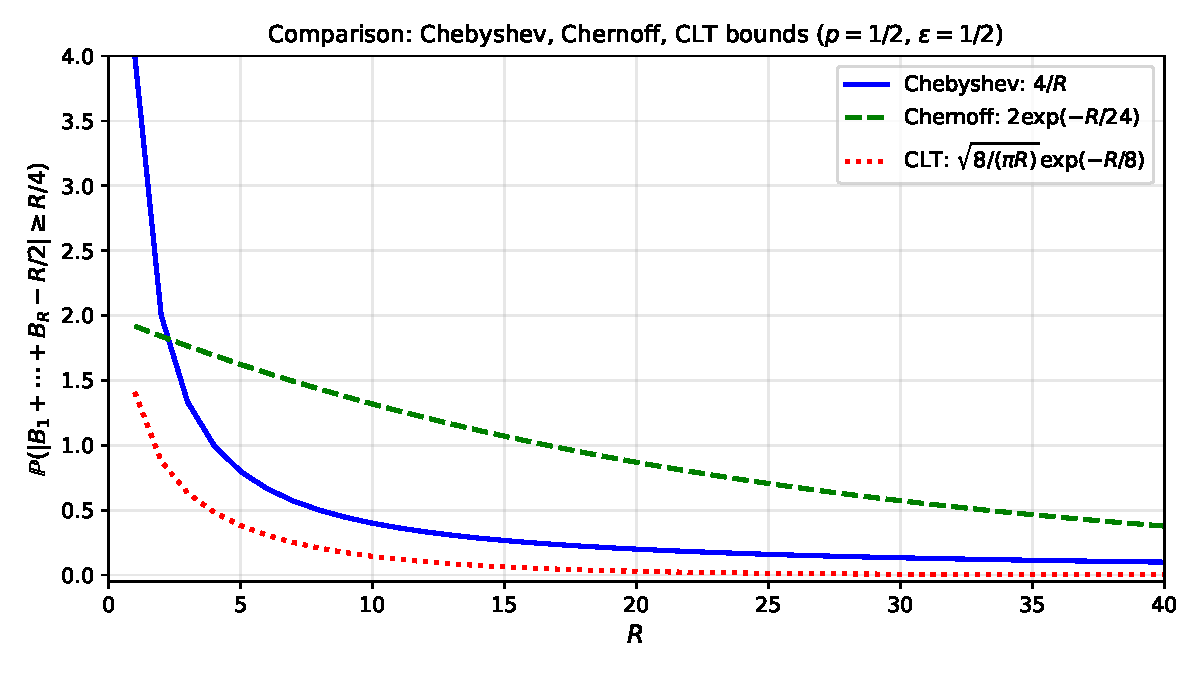
\includegraphics[width=0.75\textwidth]{fig_chernoff_comparison}
  \end{center}

  \textbf{Comparison} for $\mathbb{P}(|B_1+\cdots+B_R - R/2| \geq R/4)$, $p=1/2$, $\varepsilon = 1/2$:
  \begin{itemize}
    \item \textbf{Chebyshev}: $4/R$ (loosest, decreases slowly)
    \item \textbf{Chernoff}: $2e^{-R/24}$ (exponential decay)
    \item \textbf{CLT}: $\sqrt{8/(\pi R)}\,e^{-R/8}$ (tightest, best approximation)
  \end{itemize}

\end{frame}

%% ---- 4.4.2 Discussion on Errors
\begin{frame}[allowframebreaks]{4.4.2 Discussion on Absolute vs Relative Errors}

  \textbf{Counter-intuitive scenario:} Suppose $\mathbb{P}(Y=1) = p = 0.01$,
  $R = 1$. Then $\hat{Y}_1 = Y_1 \in \{0, 1\}$.

  \begin{itemize}
    \item $\mathbb{P}(|\hat{Y}_1 - I| \leq 0.01) = \mathbb{P}(Y_1 = 0) = 0.99$
    \item This ``satisfies'' absolute error condition (E1) with $\varepsilon = \delta = 0.01$!
    \item But relative error is huge: $|\hat{Y}_1 - I|$ is either $0.01$ or $0.99$
  \end{itemize}

  \medskip
  \textbf{Required replications ($\varepsilon = \delta = 0.01$) for \emph{absolute error}:}
  \begin{center}
    \begin{tabular}{cc}
      \toprule
      $I$ & Required $R$ \\
      \midrule
      $0.1$ & $\approx 5945$ \\
      $0.01$ & $\approx 654$ \\
      $0.001$ & $\approx 66$ \\
      \bottomrule
    \end{tabular}
  \end{center}

  Smaller $p$ $\Rightarrow$ fewer replications for absolute error!

  \framebreak

  \textbf{Required replications for \emph{relative error}} (Chernoff, $\varepsilon = \delta = 0.01$):
  \begin{center}
    \begin{tabular}{cc}
      \toprule
      $I$ & Required $R$ \\
      \midrule
      $0.1$ & $\approx 1.59 \times 10^6$ \\
      $0.01$ & $\approx 1.59 \times 10^7$ \\
      $0.001$ & $\approx 1.59 \times 10^8$ \\
      \bottomrule
    \end{tabular}
  \end{center}

  $R \propto 1/I$ for relative error -- \textbf{extremely expensive} when $I$ is small!

  \bigskip
  \begin{block}{Implication}
    When $I$ is small (e.g., rare event probability), achieving small relative error
    via naive Monte Carlo requires an impractically large number of replications.
    Variance reduction techniques (importance sampling, etc.) are essential.
  \end{block}

\end{frame}

%% ---- 4.4.3 Absolute vs Relative for pi
\begin{frame}[allowframebreaks]{4.4.3 Absolute vs Relative Error for Estimating $\pi$}

  \textbf{Setup:} Estimator $\hat{Y}_{R^{\rm abs}}$ from Example 4.1.6:
  $Y_j = 4\cdot\mathbf{1}(U_{2j-1}^2 + U_{2j}^2 \leq 1)$, $\mathbb{E}Y = \pi$,
  $\text{Var}\,Y \approx 2.6968$.

  \begin{block}{Absolute Error (CLT)}
    To achieve $\mathbb{P}(|\hat{Y}_{R^{\rm abs}} - \pi| \leq 0.01) \geq 0.99$
    ($\varepsilon = \delta = 0.01$, $z_{1-\delta/2} = 2.57$):
    \[
      R^{\rm abs} = z_{1-\delta/2}^2 \frac{\text{Var}\,Y}{\varepsilon^2}
        \approx 2.57^2 \cdot \frac{2.6968}{0.01^2} \approx 1.78 \times 10^5
    \]
  \end{block}

  \begin{block}{Relative Error (Chernoff)}
    To achieve $\mathbb{P}(|\hat{Y}_{R^{\rm rel,1}} - \pi| \leq 0.01\pi) \geq 0.99$:
    \[
      R^{\rm rel,1} \geq \frac{3\ln(2/0.01)}{0.01^2 \cdot \pi} \approx 5 \times 10^4
    \]
    \medskip
    Via CLT (setting $\varepsilon' = 0.01/\pi$): $R^{\rm rel,2} \approx 5 \times 10^5$
  \end{block}

  \begin{center}
    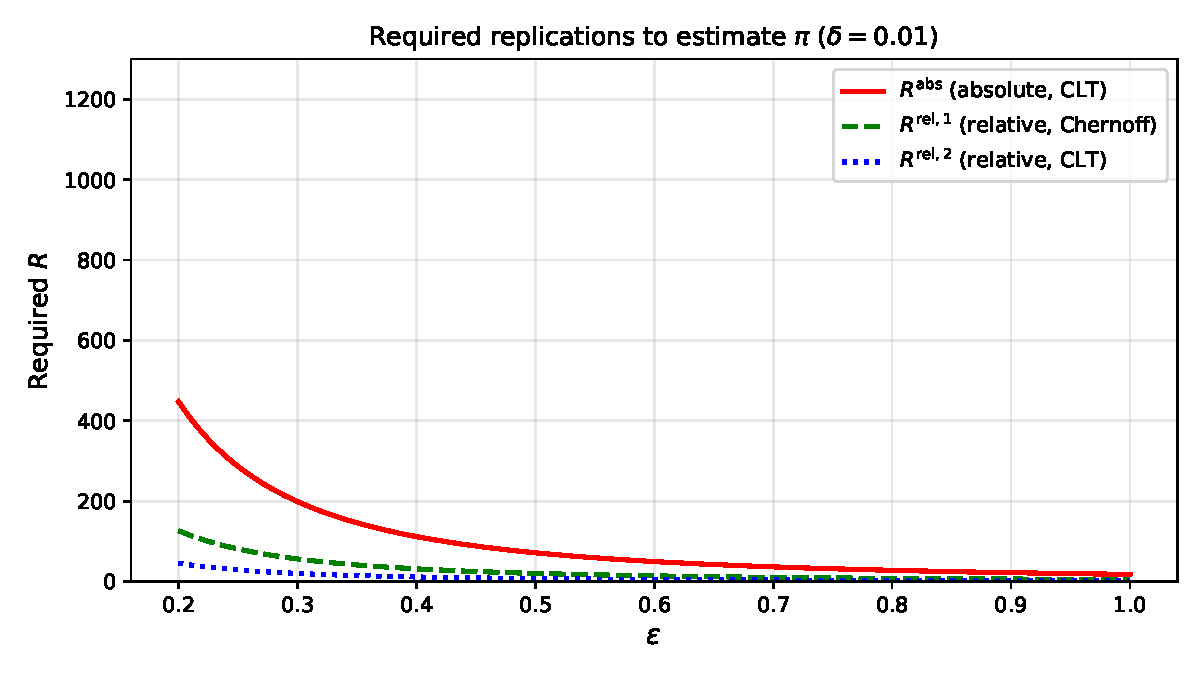
\includegraphics[width=0.70\textwidth]{fig_required_R_pi}
  \end{center}

  For $\pi \approx 3.14$, relative error requires $\sim 3\times$ more replications.

\end{frame}

%% ---- Python: Chernoff vs CLT comparison
\begin{frame}[fragile]{4.4 Python: Comparing Error Bounds}
\begin{lstlisting}[style=python]
import numpy as np
from scipy import stats

def required_R_absolute(sigma2, epsilon, delta):
    """R for absolute error via CLT."""
    z = stats.norm.ppf(1 - delta / 2)
    return z**2 * sigma2 / epsilon**2

def required_R_relative_chernoff(p, epsilon, delta):
    """R for relative error via Chernoff (Bernoulli only)."""
    return 3 * np.log(2 / delta) / (epsilon**2 * p)

def required_R_relative_clt(sigma2, I, epsilon, delta):
    """R for relative error via CLT."""
    z = stats.norm.ppf(1 - delta / 2)
    return z**2 * sigma2 / (epsilon**2 * I**2)

# Parameters for estimating pi
VarY_pi  = 16 * (np.pi/4) * (1 - np.pi/4)   # indicator estimator
I_pi     = np.pi
delta    = 0.01
epsilon  = 0.01

R_abs  = required_R_absolute(VarY_pi, epsilon, delta)
R_rel1 = required_R_relative_chernoff(np.pi/4, epsilon, delta)
R_rel2 = required_R_relative_clt(VarY_pi, I_pi, epsilon, delta)

print(f"R_abs  (absolute, CLT):     {R_abs:.2e}")
print(f"R_rel1 (relative, Chernoff):{R_rel1:.2e}")
print(f"R_rel2 (relative, CLT):     {R_rel2:.2e}")
# Output:
# R_abs  (absolute, CLT):     1.78e+05
# R_rel1 (relative, Chernoff):5.00e+04
# R_rel2 (relative, CLT):     5.02e+05
\end{lstlisting}
\end{frame}

%% ==================================================================
%% SECTION 4.5 Conclusions
%% ==================================================================

\begin{frame}[allowframebreaks]{4.5 Conclusions}

  \begin{block}{Fundamental Relationship Revisited}
    The half-width of the confidence interval satisfies:
    \[
      b = \frac{z_{1-\alpha/2}\,D}{\sqrt{R}}
    \]
    where $D$ depends on the problem:
    \begin{itemize}
      \item $I = \mathbb{E}Y$: $D = \sigma_Y$
      \item $z = k(I)$, $I = \mathbb{E}Y$: $D = |k'(I)|\,\sigma_Y$
      \item $z = k(\mathbf{I})$, $\mathbf{I} = \mathbb{E}\mathbf{Y}$: $D = \sqrt{\nabla k(\mathbf{I})\,\boldsymbol{\Sigma}_{\mathbf{Y}}\,(\nabla k(\mathbf{I}))^T}$
    \end{itemize}
  \end{block}

  \bigskip
  \textbf{Practical workflow:}
  \begin{enumerate}
    \item Run pilot simulation of size $m$ to estimate $\sigma_Y^2$ (or $\boldsymbol{\Sigma}_{\mathbf{Y}}$)
    \item Compute required $R$ from fundamental relationship
    \item Run $R$ replications; compute $\hat{Y}_R$ (or $\hat{\mathbf{Y}}_R$) and $\hat{S}_R^2$
    \item Report estimate with CI
  \end{enumerate}

  \framebreak

  \textbf{Summary of confidence intervals:}
  \begin{center}
    \begin{tabular}{lll}
      \toprule
      Quantity & Point Estimate & 95\% CI \\
      \midrule
      $I$ & $\hat{Y}_R$ & $\hat{Y}_R \pm 1.96\hat{S}_R/\sqrt{R}$ \\
      $k(I)$ & $k(\hat{Y}_R)$ & $k(\hat{Y}_R) \pm 1.96\hat{S}_R|k'(\hat{Y}_R)|/\sqrt{R}$ \\
      $q_p$ & $X_{(\lfloor pR\rfloor)}$ & $\hat{q}_p \pm 1.96\sqrt{p(1-p)/R}\hat{Q}'_{p,R}$ \\
      \bottomrule
    \end{tabular}
  \end{center}

  \bigskip
  \textbf{Key takeaways:}
  \begin{itemize}
    \item Error $b = O(R^{-1/2})$: the \textit{Monte Carlo rate}
    \item CLT gives $\approx 80\%$ fewer replications than Chebyshev for same confidence
    \item Relative error control is much harder when $I$ is small (rare events)
    \item Biased estimators: bias is $O(R^{-1})$, dominated by std.\ dev.\ $O(R^{-1/2})$ for large $R$
    \item For quantiles: $\varsigma^2 = p(1-p)/f(q_p)^2$ -- need to estimate $f(q_p)$
  \end{itemize}

\end{frame}

%% ---- Final Python example: full workflow
\begin{frame}[fragile]{4.5 Python: Full Output Analysis Workflow}
\begin{lstlisting}[style=python]
import numpy as np
from scipy import stats

def full_mc_analysis(simulate_Y, R_pilot=500, R_main=None,
                     b=0.05, alpha=0.05, seed=42):
    """Complete MC output analysis pipeline."""
    rng = np.random.default_rng(seed)

    # Step 1: Pilot simulation to estimate sigma_Y^2
    Y_pilot = np.array([simulate_Y(rng) for _ in range(R_pilot)])
    sigma2_hat = Y_pilot.var(ddof=1)
    print(f"Pilot sigma^2 estimate: {sigma2_hat:.4f}")

    # Step 2: Required R from fundamental relationship
    z = stats.norm.ppf(1 - alpha / 2)
    if R_main is None:
        R_main = int(np.ceil(z**2 * sigma2_hat / b**2))
    print(f"Required R for b={b}, alpha={alpha}: {R_main}")

    # Step 3: Main simulation
    Y_main = np.array([simulate_Y(rng) for _ in range(R_main)])
    Y_bar = Y_main.mean()
    S = Y_main.std(ddof=1)

    ci_lo = Y_bar - z * S / np.sqrt(R_main)
    ci_hi = Y_bar + z * S / np.sqrt(R_main)
    print(f"Estimate: {Y_bar:.4f}, CI: ({ci_lo:.4f}, {ci_hi:.4f})")
    return Y_bar, (ci_lo, ci_hi)

# Estimate pi: Y = 4 * 1(U1^2 + U2^2 <= 1)
def sim_pi(rng):
    u = rng.random(2)
    return 4.0 * float(u[0]**2 + u[1]**2 <= 1)

est, ci = full_mc_analysis(sim_pi, R_pilot=1000, b=0.05)
\end{lstlisting}
\end{frame}

%% ---- Summary slide
\begin{frame}{Chapter 4: Summary}
  \begin{columns}
    \begin{column}{0.48\textwidth}
      \textbf{Estimation of $I = \mathbb{E}Y$:}
      \begin{itemize}\small
        \item Unbiased estimator $\hat{Y}_R = \frac{1}{R}\sum Y_j$
        \item CLT: $\sqrt{R}(\hat{Y}_R - I) \to \mathcal{N}(0,\sigma_Y^2)$
        \item CI: $\hat{Y}_R \pm z_{1-\alpha/2}\hat{S}_R/\sqrt{R}$
        \item Required $R = z_{1-\alpha/2}^2\sigma_Y^2/b^2$
        \item 3 shapes of conf.\ regions: ellipsoid, parallelogram, rectangle
      \end{itemize}
      \medskip
      \textbf{Estimation of $k(I)$:}
      \begin{itemize}\small
        \item Delta method: $\varsigma^2 = k'(I)^2\sigma_Y^2$
        \item Generally biased; bias $= O(R^{-1})$
        \item MSE = Var + Bias$^2$
      \end{itemize}
    \end{column}
    \begin{column}{0.50\textwidth}
      \textbf{Quantile estimation:}
      \begin{itemize}\small
        \item $\hat{q}_p = X_{(\lfloor pR\rfloor)}$: consistent
        \item CLT: $\varsigma^2 = p(1-p)/f(q_p)^2$
        \item Estimate $1/f(q_p)$ via order statistics
      \end{itemize}
      \medskip
      \textbf{Error bounds:}
      \begin{itemize}\small
        \item Chebyshev: $b_R = \sigma_Y/(\alpha^{1/2}\sqrt{R})$
        \item CLT: $b = 1.96\sigma_Y/\sqrt{R}$
        \item Chernoff: exponential bound for Bernoulli
        \item CLT uses $\sim 19\%$ as many replications as Chebyshev
        \item Relative error expensive when $I$ is small
      \end{itemize}
    \end{column}
  \end{columns}

  \bigskip
  \begin{center}
    \textbf{Monte Carlo rate:} $b = O(R^{-1/2})$ regardless of dimension $d$
  \end{center}
\end{frame}

\end{document}
